\documentclass[UTF8,11pt,a4paper]{ctexart}
\usepackage[margin=2.5cm]{geometry}
\usepackage{amsmath,amssymb,booktabs,longtable,graphicx,xurl,hyperref}
\hypersetup{hidelinks}
\setCJKmainfont{Songti SC}
\setlength{\emergencystretch}{2em}
\newcommand{\RunID}{q1-20260910T142542Z}
\newcommand{\QOneCost}{35,126.9486}
\newcommand{\NoStorageCost}{48,052.0466}
\newcommand{\RuleCost}{46,428.9954}
\newcommand{\QOneGrid}{59,482.6990}
\newcommand{\Saving}{26.8981}
\newcommand{\TotalLoad}{111,024.8081}
\newcommand{\TotalPV}{55,482.8357}
\newcommand{\ChargeTotal}{20,740.6661}
\newcommand{\DischargeTotal}{16,799.9396}
\newcommand{\EfficiencyCost}{33,801.4955}
\newcommand{\PointCost}{35,042.5400}

\title{微网购电调度的确定性优化与在线预测控制}
\author{}\date{第一轮完整建模初稿，2026年9月10日}
\begin{document}\pagestyle{plain}\maketitle
\begin{abstract}
基于本地赛题与全量附件，构建10分钟调度网格，以母线电量、内部储能和合同账本分离的方式研究微网购电。在暂定单程充放电效率90\%和区间平均功率解释下，确定性MILP的购电费用为\QOneCost 元，较无储能节省\Saving\%，求解器最优间隙为零并与同约束LP下界一致。对2025年2月至12月334日，采用历史滚动选模、净负载误差裕量和区间内反馈模拟，进一步比较日前预测、发布预报、合同修改及波动价格下的13种预设策略。额外预报在当前控制器中并非必然降低样本费用；退款口径会改变策略比较。所有结果均来自可复现代码，原件哈希不变，未使用未来真值制定日前计划。实时观测聚合近似、模板时间错位及结算解释仍需最终核验，不能将本初稿视为已完成官方语义与人工审核的提交稿。
\end{abstract}
\noindent\textbf{关键词：}混合整数线性规划；因果预测；储能控制；合同结算；信息边界
\clearpage

\section{问题重述与模型递进}
题面\cite{problem}第一问在已给日电价、负载和光伏预测下于0点制定购电计划，储能首末相等。第二问只能用历史负载和光伏预测未来，普通计划全额计费，缺口以五倍电价紧急购买。第三问加入0、6、12、18点发布的未来24个整点光伏预测和增减合同费用，需评价预报与修改机会。第四问用实时波动电价重算第二、三问，未来价格是否预先已知未明确。

路线为数据审计、确定性物理基线、历史预测与误差决策、因果模拟、预报版本和合同事件、波动价扩展。既有蒸馏知识主要提供接口、硬约束复算、全知与在线结果区分等审计经验，并未转用历史数值、参数或未经核验的奖项结论。

\section{数据检查与假设}
完整检查3页题面、4个数据工作簿和5个结果模板。附件2和4均为365日乘144时段，附件3有1460次发布和35040个整点预测值；数值无缺失或负值，波动价范围0.0076--1.7936元/kWh。附件3的省写日期前填仅恢复表结构，不填补数值。11份原件的迁移前后SHA-256一致，原始字节不变。

内部区间为$[t/6,(t+1)/6)$小时，每日144区间和145状态端点。原始00:10--24:00标签暂解释为此前10分钟平均功率或交付价，$e=P/6$；题面未明确平均/瞬时，另作Q1瞬时周期端点积分敏感性。模板购电标签整体晚10分钟，原格式保留并提供逐格映射，导出文件标记语义待澄清。

采用交流侧充电$c$、放电$d$，电池内部状态$E$，单程效率均0.9、功率限5000kW、内部电量界1200--10800kWh。第一问首末6000kWh；后续从1月1日6000开始，1月电池停用预热，2月后跨日承接，不每日重置。无售电，富余可不用，未利用已购电不退费；紧急电只填负载缺口，不充电。

实时执行以本区间平均功率作为区间内恒定代表值反馈平衡。它不是在区间起点获知后来才完成的实测总量，亦不证明现场动态可实施性。日前规划只见截至决策时已完成标签；训练、缩放、模型选择和残差校准均保留时间边界。

\section{第一问：确定性MILP}
设$q_t,w_t$分别为普通购电和总未利用电量，$\ell_t,v_t$为负载和光伏电量，$p_t$为电价，$z_t$控制互斥。模型为
\begin{align}
\min\ &\sum_t p_tq_t, &q_t+v_t+d_t&=\ell_t+c_t+w_t,\\
E_{t+1}&=E_t+0.9c_t-d_t/0.9, &1200&\le E_t\le10800,\\
0&\le c_t\le(5000/6)z_t, &0&\le d_t\le(5000/6)(1-z_t),\\
q_t,w_t&\ge0,\quad z_t\in\{0,1\}, &E_0&=E_{144}=6000.
\end{align}
用SciPy/HiGHS\cite{scipy}求解，同时运行无储能、低价充高价放规则和其余约束相同但放松二元变量的LP下界。本例LP解另经互斥检查通过。MILP费用\QOneCost 元、计划购电\QOneGrid kWh，充电\ChargeTotal kWh、放电\DischargeTotal kWh，未利用电量为0。无储能费用\NoStorageCost 元，规则费用\RuleCost 元。

\begin{center}\small\begin{tabular}{lrlrlr}\toprule 时间段 & 购电量 & 时间段 & 购电量 & 时间段 & 购电量\\\midrule
10:00--10:10 & 0.0000 & 12:00--12:10 & 480.4124 & 14:00--14:10 & 0.0000\\
16:00--16:10 & 445.4316 & 18:00--18:10 & 531.8940 & 20:00--20:10 & 0.0000\\
\midrule\multicolumn{2}{c}{全天购电量/kWh} & 59,482.6990 & \multicolumn{2}{c}{全天购电费/元} & 35,126.9486\\
\bottomrule\end{tabular}
\par\medskip\small\begin{tabular}{lrrlrr}\toprule 时间段 & 充电量 & 放电量 & 时间段 & 充电量 & 放电量\\\midrule
0:00--4:00 & 4500.0000 & 0.0000 & 4:00--8:00 & 833.3333 & 6365.8412\\
8:00--12:00 & 4787.9643 & 1702.9970 & 12:00--16:00 & 5286.0352 & 91.1014\\
16:00--20:00 & 0.0000 & 5780.1319 & 20:00--24:00 & 5333.3333 & 2859.8681\\
\midrule\multicolumn{2}{c}{0:00储电量} & 6000 & \multicolumn{2}{c}{24:00储电量} & 6000\\
\bottomrule\end{tabular}
\end{center}
全局最低价05:30--05:40确实充到10800kWh。午间12:40保留1656.2079kWh内部空间，恰好容纳随后至14:30的1840.231kWh净光伏乘0.9，不能机械断言最低价总要充满或总不充满。

HiGHS返回optimal和gap=0，MILP与LP下界一致。独立母线残差约$1.14\times10^{-13}$kWh、SOC递推残差约$8.60\times10^{-13}$kWh；首末、功率、上下界、互斥、费用与模板读回均通过。若单程效率改为$\sqrt{0.9}$，费用\EfficiencyCost 元；若功率为周期瞬时端点线性积分，费用\PointCost 元。它们是独立解释实验，不替代主结果。
\begin{figure}[htbp]\centering
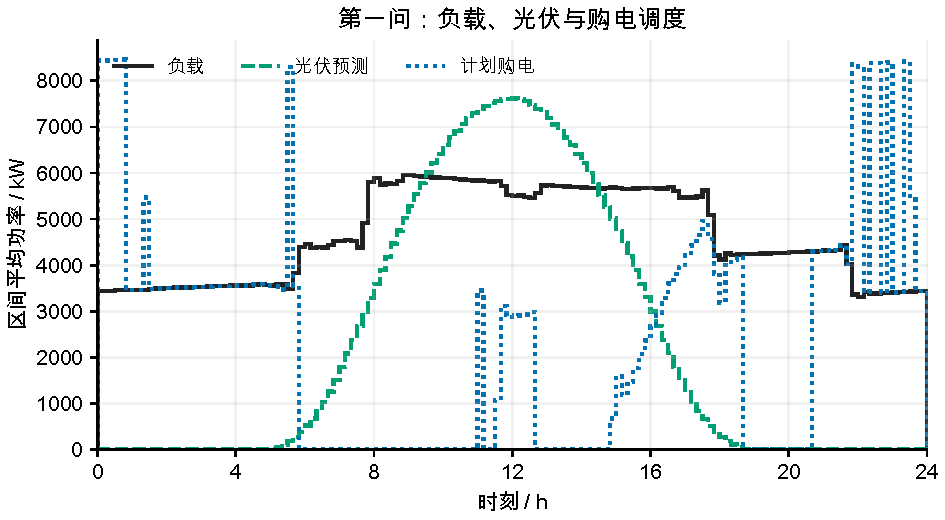
\includegraphics[width=0.92\linewidth]{../../figures/q1/q1_dispatch.pdf}
\caption{第一问真实调度，区间kWh乘6换算为平均kW，无平滑。}
\end{figure}
\begin{figure}[htbp]\centering
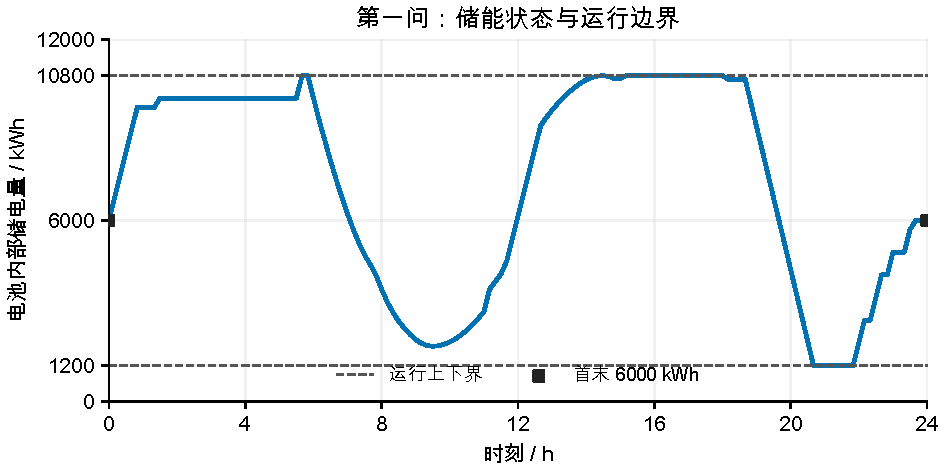
\includegraphics[width=0.92\linewidth]{../../figures/q1/q1_soc.pdf}
\caption{第一问145个内部状态端点及运行界。上午放电与午间留容对应后续光伏。}
\end{figure}

\section{第二问：历史预测、误差裕量与执行}
每个0点仅向ForecastProvider传入已完成历史快照。预测候选为昨日同刻、上周同刻和Ridge回归。回归使用昨日/上周/过去7日均值、日周期正余弦和周末特征，训练窗口最多60日，标准化仅用训练折，Ridge正则系数固定10。用此前14个已完成日的候选样本外均方误差分别选择负载和光伏预测，不用全年测试成绩倒选模型。

记此前样本外净负载残差$r=\ell-v-\widehat\ell+\widehat v$。安全裕量按4小时组在最多28个历史日估计；分位候选0.5、0.65、0.8、0.9、0.95，在至少14日残差时用最后7个历史日检验代理费用$p[b+5(r-b)_+]$，否则采用预先定义的0.8冷启动。该代理没有完整重放储能经济影响，故不称随机优化最优。

日前用$\widehat\ell+b,\widehat v$求解物理优化，规划终端目标6000kWh用于抑制末端放空，并非每日实际强制回到该值。实际电量不平衡时，当前区间有盈余便在功率/容量允许下充电；不足时按参考下一状态保留能量并放电，剩余缺口紧急购买。另以可用电池优先消缺的贪心控制作为预设对照。紧急电与充电不同时发生。

第二问结算为$C=\sum p_tq_t+\sum5p_tu_t$；原计划未利用也全付。普通合同、实际利用和紧急电分列，未利用光伏与未利用已购电按明确的光伏优先约定分开统计。
\begin{figure}[htbp]\centering
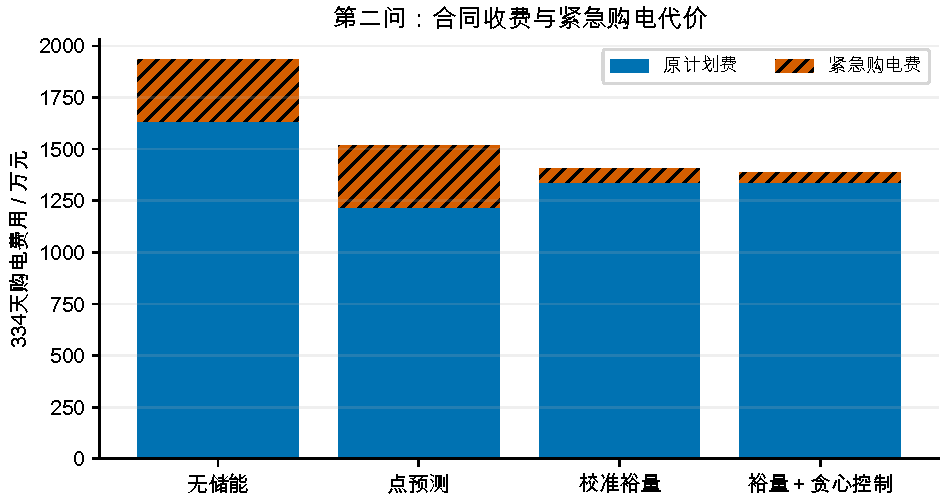
\includegraphics[width=0.92\linewidth]{../../figures/q2/q2_cost.pdf}
\caption{第二问预设策略的334日合同和紧急费用，无需将低预测误差直接等同低调度费用。}
\end{figure}

\section{第三问：预报版本、滚动控制和事件账本}
附件3保存issue time、available at、target time、lead time和value，不按目标时刻覆盖版本。预报为lead1--24整点，lead0暂用上一个已完成区间PV平均功率作代理，非负分段线性重构并积分到10分钟。0点和6/12/18点只读取当时已经发布的版本。日内负载仍用零点预测和历史校准裕量；零点版本残差裕量沿用至日内，是尚待分提前期改进的近似。

6/12/18点冻结已交付合同，重算剩余时段；固定合同的候选始终存在。因固定合同可能无法补足终端储能，日内使用终端短缺软罚$\lambda(6000-E_T)_+$，其中$\lambda=\min p/0.9$，不允许紧急电给电池充电。采用相同日内重优化机会但冻结零点预报的对照，控制终端形式与重优化的混杂。

以下先写单次调整：原合同$q^0$调整为$a$时，$\Delta^+=(a-q^0)_+$，$\Delta^-=(q^0-a)_+$。题面退款未消歧，分别计算
\begin{align}
C_A&=pq^0+1.5p\Delta^++0.5p\Delta^-+5pu,\\
C_B&=pq^0+1.5p\Delta^+-0.5p\Delta^-+5pu.
\end{align}
多次修改暂按最近合同产生事件并累计，原费只收一次。B的减量退款为原价、另收50\%罚，先增后减仍有净成本，不能制造套利。A在正价且可不用富余时纯减购被不改弱支配。

比较仅零点、冻结预报重规划、四预报仅更新电池、四预报允许修改A、选择性修改A及B敏感性。选择性A仅在预期改善超过当时价格乘历史裕量之和时改购，阈值未按全期成绩调优。实际结果不保证每次新信息或修改都有样本收益。

\section{第四问：波动价格的信息边界}
附件4未提供价格发布机制，主结果将未来真实价留给事后结算，规划用已完成历史的价格候选预测。固定/波动价格与历史/发布PV共用四类独立校准器；波动价裕量用历史实际价格与残差配对计算代理损失，不将相关项擅自拆成独立期望。修改增减费和紧急费均以实际交付区间价独立重算。提前知道全日电价不是本轮正式主结果的信息条件。

\section{全评估期结果、指定日与解释}
以下全部是同一个最终源码快照运行的334日结果，每策略48096区间。初始6000，实际终态在表中明列。修改次数指有非零合同变化的决策次数，不是电池反馈次数。
\small\begin{longtable}{lrrrr}\toprule 策略 & 费用/万元 & 紧急电/MWh & 末储量/kWh & 修改次数\\\midrule\endfirsthead
\toprule 策略 & 费用/万元 & 紧急电/MWh & 末储量/kWh & 修改次数\\\midrule\endhead
Q2无储能 & 1932.89 & 752.42 & 6000.00 & 0\\
Q2点预测 & 1518.74 & 658.47 & 5929.38 & 0\\
Q2校准裕量 & 1405.62 & 148.12 & 6064.78 & 0\\
Q2裕量与贪心 & 1387.57 & 79.79 & 6038.53 & 0\\
Q3仅零点预报 & 1431.56 & 162.69 & 6164.79 & 0\\
Q3冻结预报重规划 & 1431.35 & 163.63 & 6164.79 & 0\\
Q3四预报仅电池 & 1490.33 & 311.73 & 6164.79 & 0\\
Q3允许调整A & 1439.56 & 69.30 & 6164.79 & 431\\
Q3选择性调整A & 1439.75 & 99.78 & 6164.79 & 130\\
Q3允许调整B & 1422.56 & 96.18 & 6164.79 & 890\\
Q4-2因果价格 & 1482.98 & 134.17 & 6087.42 & 0\\
Q4-3调整A & 1521.37 & 66.80 & 6187.39 & 419\\
Q4-3调整B & 1506.13 & 93.15 & 6187.39 & 934\\
\bottomrule\end{longtable}

第二问校准裕量比点预测少支出约113.11万元，但单日并非总获益。贪心控制对照较裕量参考轨迹更低费用，不据此在全年结束后重新定义正式策略或声称最优。

第三问四预报仅更新电池比冻结预报同机会重规划多589835.34元。允许调整A比同四预报电池对照节省507689.80元，但仍比仅零点预报贵。当前利用方式没有证明其他时刻预报必须引入；额外信息理论上可以忽略，因此这个不利结果不能解释为信息自身负价值。B结果与A不同依赖退款口径，不能混合排名后宣称统一最优。

指定日期总费用含原计划、累计修改、退款及紧急费用；计划电量仅为0点原合同，二者口径不同。全部144区间、每4小时充放以及紧急事件均保存在对应工作簿与源明细，以下为指定日摘要。
\small\begin{longtable}{llrrrr}\toprule 策略 & 日期 & 原计划/kWh & 紧急电/kWh & 总费/元 & 末储量/kWh\\\midrule\endfirsthead
\toprule 策略 & 日期 & 原计划/kWh & 紧急电/kWh & 总费/元 & 末储量/kWh\\\midrule\endhead
Q2校准裕量 & 03-20 & 73586.8 & 102.4 & 45685.5 & 7036.2\\
Q2校准裕量 & 06-21 & 34165.8 & 344.5 & 20345.7 & 6598.7\\
Q2校准裕量 & 09-23 & 74361.8 & 185.2 & 47700.3 & 7646.6\\
Q2校准裕量 & 12-21 & 94287.5 & 727.2 & 63259.7 & 6143.4\\
Q3允许调整A & 03-20 & 72997.6 & 37.9 & 45950.1 & 7007.5\\
Q3允许调整A & 06-21 & 35399.5 & 0.0 & 20346.9 & 7314.7\\
Q3允许调整A & 09-23 & 73916.3 & 11.3 & 46522.9 & 6919.0\\
Q3允许调整A & 12-21 & 98660.4 & 74.6 & 64629.7 & 6551.1\\
Q4-2因果价格 & 03-20 & 73294.5 & 94.9 & 46902.0 & 7204.9\\
Q4-2因果价格 & 06-21 & 34429.3 & 320.9 & 17732.4 & 6677.9\\
Q4-2因果价格 & 09-23 & 74357.2 & 142.6 & 49640.7 & 7959.3\\
Q4-2因果价格 & 12-21 & 94425.5 & 655.1 & 73903.2 & 6163.7\\
Q4-3调整A & 03-20 & 72596.0 & 33.2 & 47179.2 & 7265.2\\
Q4-3调整A & 06-21 & 35671.9 & 0.0 & 17931.8 & 7407.8\\
Q4-3调整A & 09-23 & 73838.5 & 0.0 & 48544.0 & 7088.8\\
Q4-3调整A & 12-21 & 98827.8 & 153.0 & 76311.2 & 6588.6\\
\bottomrule\end{longtable}


\section{验证、稳健性与局限}
18项Q1解析/极端/实际重算测试及在线测试覆盖常价、无PV、零负载、容量功率界、时段计量、未来扰动、预报版本、合同100改80/120、不变与多次修改。独立审计不复用生产验证器，逐步重算全部13策略的SOC、母线、费用和事件合同，核验原件、源码和输入哈希。修改未来不可见真值或未来预报不改变过去计划及已发生调整，事后结算随真实价格变化属于预期。

配对费用差和7日移动块2000次再抽样描述区间保存在结果表中；单年季节数据的再抽样不是未来年保证。Q1效率/采样敏感性已执行，A/B账本敏感性已执行；价格已知条件、严格观测延迟、逐lead预报误差校准及容量功率研究性改变尚未完成，均不预填收益。

限制包括区间内平均功率反馈近似、PV lead0代理、日内沿用零点裕量、点预测规划与终端短缺启发式、结算和时间标签歧义。求解器对每次给定输入优化最优，不代表整套在线策略随机全局最优；自动核验不等于现场独立验证或队员人工审查。

\section*{AI工具使用声明}
Codex参与材料/技能审计、模型和假设建议、编程、真实实验、验证、图表与本初稿。依照官方规定\cite{ai}，具体部署版本待据实际界面补全，未虚构人工审核；参赛队须逐项审查核心成果。完整使用详情单独保存为PDF。
\begin{thebibliography}{9}
\bibitem{problem} 2026年高教社杯全国大学生数学建模竞赛C题：微网与外部电网电力调控策略. 2026. 题面及附件1--5.
\bibitem{scipy} SciPy社区. scipy.optimize.milp：在线软件文档[EB/OL]. 访问日期：2026-09-10. \url{https://docs.scipy.org/doc/scipy/reference/generated/scipy.optimize.milp.html}.
\bibitem{ai} 全国大学生数学建模竞赛组委会. 全国大学生数学建模竞赛人工智能工具使用规定（2026年试行）[EB/OL]. 2026-08-03. \url{https://www.mcm.edu.cn/html_cn/node/fef94648f2836ab6cc81586f4c38512b.html}.
\end{thebibliography}
\section*{支撑材料}
赛题及原附件是主要输入，保留原路径迁移清单和哈希。官方AI使用规范已保存来源PDF。历史知识库仅用作内部方法审计，不将未核奖级作为方法正确性证据。完整可运行源码、依赖锁、配置、运行指纹、原始模板、逐区间数据、各项检验和图表源路径均见README与CLAIM\_EVIDENCE\_MAP；本初稿不替代最终按竞赛格式整合源码附录和支撑包。
\clearpage
\appendix
\clearpage
\section{指定日期的分时购电、储能与紧急事件}
\label{sec:designated_details}
\subsection{第二问：校准裕量方案，2025-03-20}
\begingroup\small
\setlength{\tabcolsep}{4pt}\renewcommand{\arraystretch}{1.08}
\setlength{\LTpre}{4pt}\setlength{\LTpost}{4pt}
\noindent 购电量均为最终普通合同量加紧急购电量，包含已付费但未利用的合同电量；不等同于实际利用电量。时间使用内部当日标准网格，所有电量单位为kWh，费用单位为元。
\begin{center}\textbf{表1\quad 指定时段购电量与全天购电量、购电费}\par\smallskip
\begin{tabular}{lr lr lr}\toprule
时间段 & 购电量 & 时间段 & 购电量 & 时间段 & 购电量\\\midrule
10:00--10:10 & 0.000000 & 12:00--12:10 & 646.321116 & 14:00--14:10 & 0.000000\\
16:00--16:10 & 562.261550 & 18:00--18:10 & 725.039414 & 20:00--20:10 & 0.000000\\
\midrule
\multicolumn{2}{l}{全天购电量} & 73689.189850 & \multicolumn{2}{l}{全天购电费} & 45685.509147\\
\bottomrule\end{tabular}\end{center}
\noindent 0点原计划量：73586.792976；最终普通合同量：73586.792976；紧急量：102.396874。
全天费用含原计划费45296.903293、增购费0.000000、减购违约费0.000000、退款扣减0.000000及紧急费388.605854。
\begin{center}\textbf{表2\quad 指定时段充放电量与0点、24点储电量}\par\smallskip
\begin{tabular}{lrr lrr}\toprule
时间段 & 充电量 & 放电量 & 时间段 & 充电量 & 放电量\\\midrule
00:00--04:00 & 3888.738347 & 61.061316 & 04:00--08:00 & 1395.424924 & 4434.706034\\
08:00--12:00 & 6291.457017 & 2777.377217 & 12:00--16:00 & 1887.887545 & 254.722783\\
16:00--20:00 & 0.000000 & 5191.426212 & 20:00--24:00 & 5844.723643 & 2930.216483\\
\midrule
\multicolumn{2}{l}{0:00储电量} & 7047.140007 & \multicolumn{2}{l}{24:00储电量} & 7036.203839\\
\bottomrule\end{tabular}\end{center}
\noindent 充电、放电分别为交流母线侧输入、输出；储电量为电池内部状态。同一四小时段可分别发生充电和放电，逐10分钟区间保持互斥。
\begin{center}\textbf{表3\quad 当日全部紧急购电事件}\end{center}
\begin{longtable}{llr}\toprule 日期 & 紧急购电时间段 & 紧急购电量\\\midrule\endfirsthead
\toprule 日期 & 紧急购电时间段 & 紧急购电量\\\midrule\endhead
\bottomrule\endfoot
2025-03-20 & 01:20--01:30 & 16.616961\\
 & 15:50--16:20 & 85.779912\\
\midrule\multicolumn{2}{l}{当日事件电量合计} & 102.396874\\
\end{longtable}
\noindent 事件阈值为$10^{-7}$kWh；连续超阈值区间合并，不跨零值、不跨日。
\endgroup
\clearpage
\subsection{第二问：校准裕量方案，2025-06-21}
\begingroup\small
\setlength{\tabcolsep}{4pt}\renewcommand{\arraystretch}{1.08}
\setlength{\LTpre}{4pt}\setlength{\LTpost}{4pt}
\noindent 购电量均为最终普通合同量加紧急购电量，包含已付费但未利用的合同电量；不等同于实际利用电量。时间使用内部当日标准网格，所有电量单位为kWh，费用单位为元。
\begin{center}\textbf{表1\quad 指定时段购电量与全天购电量、购电费}\par\smallskip
\begin{tabular}{lr lr lr}\toprule
时间段 & 购电量 & 时间段 & 购电量 & 时间段 & 购电量\\\midrule
10:00--10:10 & 0.000000 & 12:00--12:10 & 0.000000 & 14:00--14:10 & 0.000000\\
16:00--16:10 & 157.793481 & 18:00--18:10 & 0.000000 & 20:00--20:10 & 0.000000\\
\midrule
\multicolumn{2}{l}{全天购电量} & 34510.372468 & \multicolumn{2}{l}{全天购电费} & 20345.692461\\
\bottomrule\end{tabular}\end{center}
\noindent 0点原计划量：34165.835272；最终普通合同量：34165.835272；紧急量：344.537196。
全天费用含原计划费19263.957020、增购费0.000000、减购违约费0.000000、退款扣减0.000000及紧急费1081.735440。
\begin{center}\textbf{表2\quad 指定时段充放电量与0点、24点储电量}\par\smallskip
\begin{tabular}{lrr lrr}\toprule
时间段 & 充电量 & 放电量 & 时间段 & 充电量 & 放电量\\\midrule
00:00--04:00 & 312.530350 & 374.359401 & 04:00--08:00 & 375.733136 & 4218.162247\\
08:00--12:00 & 10185.760390 & 0.000000 & 12:00--16:00 & 0.000000 & 0.000000\\
16:00--20:00 & 51.383831 & 5904.763402 & 20:00--24:00 & 5799.093867 & 2615.313917\\
\midrule
\multicolumn{2}{l}{0:00储电量} & 6116.180343 & \multicolumn{2}{l}{24:00储电量} & 6598.677352\\
\bottomrule\end{tabular}\end{center}
\noindent 充电、放电分别为交流母线侧输入、输出；储电量为电池内部状态。同一四小时段可分别发生充电和放电，逐10分钟区间保持互斥。
\begin{center}\textbf{表3\quad 当日全部紧急购电事件}\end{center}
\begin{longtable}{llr}\toprule 日期 & 紧急购电时间段 & 紧急购电量\\\midrule\endfirsthead
\toprule 日期 & 紧急购电时间段 & 紧急购电量\\\midrule\endhead
\bottomrule\endfoot
2025-06-21 & 00:20--00:30 & 10.332555\\
 & 02:00--02:10 & 3.137279\\
 & 02:20--02:30 & 5.684046\\
 & 02:50--03:30 & 89.644241\\
 & 04:10--04:20 & 5.006413\\
 & 04:50--05:20 & 86.636956\\
 & 05:40--06:30 & 120.772110\\
 & 17:30--17:50 & 23.323597\\
\midrule\multicolumn{2}{l}{当日事件电量合计} & 344.537196\\
\end{longtable}
\noindent 事件阈值为$10^{-7}$kWh；连续超阈值区间合并，不跨零值、不跨日。
\endgroup
\clearpage
\subsection{第二问：校准裕量方案，2025-09-23}
\begingroup\small
\setlength{\tabcolsep}{4pt}\renewcommand{\arraystretch}{1.08}
\setlength{\LTpre}{4pt}\setlength{\LTpost}{4pt}
\noindent 购电量均为最终普通合同量加紧急购电量，包含已付费但未利用的合同电量；不等同于实际利用电量。时间使用内部当日标准网格，所有电量单位为kWh，费用单位为元。
\begin{center}\textbf{表1\quad 指定时段购电量与全天购电量、购电费}\par\smallskip
\begin{tabular}{lr lr lr}\toprule
时间段 & 购电量 & 时间段 & 购电量 & 时间段 & 购电量\\\midrule
10:00--10:10 & 0.000000 & 12:00--12:10 & 488.351540 & 14:00--14:10 & 0.000000\\
16:00--16:10 & 589.432650 & 18:00--18:10 & 819.707702 & 20:00--20:10 & 3.670570\\
\midrule
\multicolumn{2}{l}{全天购电量} & 74547.083841 & \multicolumn{2}{l}{全天购电费} & 47700.328683\\
\bottomrule\end{tabular}\end{center}
\noindent 0点原计划量：74361.835161；最终普通合同量：74361.835161；紧急量：185.248680。
全天费用含原计划费46890.370816、增购费0.000000、减购违约费0.000000、退款扣减0.000000及紧急费809.957867。
\begin{center}\textbf{表2\quad 指定时段充放电量与0点、24点储电量}\par\smallskip
\begin{tabular}{lrr lrr}\toprule
时间段 & 充电量 & 放电量 & 时间段 & 充电量 & 放电量\\\midrule
00:00--04:00 & 3873.470074 & 0.000000 & 04:00--08:00 & 265.399059 & 5202.241497\\
08:00--12:00 & 6003.948130 & 1896.615717 & 12:00--16:00 & 2854.563205 & 291.510206\\
16:00--20:00 & 0.000000 & 5252.206620 & 20:00--24:00 & 6306.804725 & 2694.322999\\
\midrule
\multicolumn{2}{l}{0:00储电量} & 7313.876933 & \multicolumn{2}{l}{24:00储电量} & 7646.646899\\
\bottomrule\end{tabular}\end{center}
\noindent 充电、放电分别为交流母线侧输入、输出；储电量为电池内部状态。同一四小时段可分别发生充电和放电，逐10分钟区间保持互斥。
\begin{center}\textbf{表3\quad 当日全部紧急购电事件}\end{center}
\begin{longtable}{llr}\toprule 日期 & 紧急购电时间段 & 紧急购电量\\\midrule\endfirsthead
\toprule 日期 & 紧急购电时间段 & 紧急购电量\\\midrule\endhead
\bottomrule\endfoot
2025-09-23 & 14:20--15:00 & 180.024633\\
 & 16:00--16:10 & 5.224047\\
\midrule\multicolumn{2}{l}{当日事件电量合计} & 185.248680\\
\end{longtable}
\noindent 事件阈值为$10^{-7}$kWh；连续超阈值区间合并，不跨零值、不跨日。
\endgroup
\clearpage
\subsection{第二问：校准裕量方案，2025-12-21}
\begingroup\small
\setlength{\tabcolsep}{4pt}\renewcommand{\arraystretch}{1.08}
\setlength{\LTpre}{4pt}\setlength{\LTpost}{4pt}
\noindent 购电量均为最终普通合同量加紧急购电量，包含已付费但未利用的合同电量；不等同于实际利用电量。时间使用内部当日标准网格，所有电量单位为kWh，费用单位为元。
\begin{center}\textbf{表1\quad 指定时段购电量与全天购电量、购电费}\par\smallskip
\begin{tabular}{lr lr lr}\toprule
时间段 & 购电量 & 时间段 & 购电量 & 时间段 & 购电量\\\midrule
10:00--10:10 & 0.000000 & 12:00--12:10 & 930.854308 & 14:00--14:10 & 0.000000\\
16:00--16:10 & 803.069923 & 18:00--18:10 & 720.824933 & 20:00--20:10 & 0.000000\\
\midrule
\multicolumn{2}{l}{全天购电量} & 95014.616246 & \multicolumn{2}{l}{全天购电费} & 63259.717029\\
\bottomrule\end{tabular}\end{center}
\noindent 0点原计划量：94287.458657；最终普通合同量：94287.458657；紧急量：727.157589。
全天费用含原计划费60272.344434、增购费0.000000、减购违约费0.000000、退款扣减0.000000及紧急费2987.372595。
\begin{center}\textbf{表2\quad 指定时段充放电量与0点、24点储电量}\par\smallskip
\begin{tabular}{lrr lrr}\toprule
时间段 & 充电量 & 放电量 & 时间段 & 充电量 & 放电量\\\midrule
00:00--04:00 & 4673.807151 & 141.266533 & 04:00--08:00 & 1743.473158 & 1570.546592\\
08:00--12:00 & 5375.247137 & 7516.412716 & 12:00--16:00 & 7673.957141 & 2220.109417\\
16:00--20:00 & 0.000000 & 5713.535250 & 20:00--24:00 & 5475.586030 & 2912.610677\\
\midrule
\multicolumn{2}{l}{0:00储电量} & 6000.536378 & \multicolumn{2}{l}{24:00储电量} & 6143.420842\\
\bottomrule\end{tabular}\end{center}
\noindent 充电、放电分别为交流母线侧输入、输出；储电量为电池内部状态。同一四小时段可分别发生充电和放电，逐10分钟区间保持互斥。
\begin{center}\textbf{表3\quad 当日全部紧急购电事件}\end{center}
\begin{longtable}{llr}\toprule 日期 & 紧急购电时间段 & 紧急购电量\\\midrule\endfirsthead
\toprule 日期 & 紧急购电时间段 & 紧急购电量\\\midrule\endhead
\bottomrule\endfoot
2025-12-21 & 01:00--01:20 & 30.519780\\
 & 01:30--01:50 & 49.949628\\
 & 02:00--02:20 & 40.838567\\
 & 03:30--04:20 & 150.259727\\
 & 05:40--06:40 & 140.095317\\
 & 07:50--08:00 & 44.083698\\
 & 12:50--13:10 & 51.930062\\
 & 15:50--16:00 & 10.061285\\
 & 16:20--16:30 & 8.780842\\
 & 16:50--17:00 & 13.875000\\
 & 17:20--17:30 & 8.866667\\
 & 18:10--19:00 & 153.774817\\
 & 19:50--20:00 & 24.122200\\
\midrule\multicolumn{2}{l}{当日事件电量合计} & 727.157589\\
\end{longtable}
\noindent 事件阈值为$10^{-7}$kWh；连续超阈值区间合并，不跨零值、不跨日。
\endgroup
\clearpage
\subsection{第三问：允许调整，A口径，2025-03-20}
\begingroup\small
\setlength{\tabcolsep}{4pt}\renewcommand{\arraystretch}{1.08}
\setlength{\LTpre}{4pt}\setlength{\LTpost}{4pt}
\noindent 购电量均为最终普通合同量加紧急购电量，包含已付费但未利用的合同电量；不等同于实际利用电量。时间使用内部当日标准网格，所有电量单位为kWh，费用单位为元。
\begin{center}\textbf{表1\quad 指定时段购电量与全天购电量、购电费}\par\smallskip
\begin{tabular}{lr lr lr}\toprule
时间段 & 购电量 & 时间段 & 购电量 & 时间段 & 购电量\\\midrule
10:00--10:10 & 0.000000 & 12:00--12:10 & 621.759387 & 14:00--14:10 & 0.000000\\
16:00--16:10 & 673.949918 & 18:00--18:10 & 749.273161 & 20:00--20:10 & 0.000000\\
\midrule
\multicolumn{2}{l}{全天购电量} & 73540.019023 & \multicolumn{2}{l}{全天购电费} & 45950.085363\\
\bottomrule\end{tabular}\end{center}
\noindent 0点原计划量：72997.572689；最终普通合同量：73502.118547；紧急量：37.900476。
全天费用含原计划费45258.297047、增购费610.608196、减购违约费0.000000、退款扣减0.000000及紧急费81.180120。
\begin{center}\textbf{表2\quad 指定时段充放电量与0点、24点储电量}\par\smallskip
\begin{tabular}{lrr lrr}\toprule
时间段 & 充电量 & 放电量 & 时间段 & 充电量 & 放电量\\\midrule
00:00--04:00 & 3800.991467 & 78.256984 & 04:00--08:00 & 793.709005 & 5441.462900\\
08:00--12:00 & 5708.486487 & 2777.377217 & 12:00--16:00 & 4481.146104 & 254.722783\\
16:00--20:00 & 0.000000 & 5137.116104 & 20:00--24:00 & 5750.841348 & 2934.286889\\
\midrule
\multicolumn{2}{l}{0:00储电量} & 6996.122337 & \multicolumn{2}{l}{24:00储电量} & 7007.531665\\
\bottomrule\end{tabular}\end{center}
\noindent 充电、放电分别为交流母线侧输入、输出；储电量为电池内部状态。同一四小时段可分别发生充电和放电，逐10分钟区间保持互斥。
\begin{center}\textbf{表3\quad 当日全部紧急购电事件}\end{center}
\begin{longtable}{llr}\toprule 日期 & 紧急购电时间段 & 紧急购电量\\\midrule\endfirsthead
\toprule 日期 & 紧急购电时间段 & 紧急购电量\\\midrule\endhead
\bottomrule\endfoot
2025-03-20 & 01:10--01:40 & 37.900476\\
\midrule\multicolumn{2}{l}{当日事件电量合计} & 37.900476\\
\end{longtable}
\noindent 事件阈值为$10^{-7}$kWh；连续超阈值区间合并，不跨零值、不跨日。
\endgroup
\clearpage
\subsection{第三问：允许调整，A口径，2025-06-21}
\begingroup\small
\setlength{\tabcolsep}{4pt}\renewcommand{\arraystretch}{1.08}
\setlength{\LTpre}{4pt}\setlength{\LTpost}{4pt}
\noindent 购电量均为最终普通合同量加紧急购电量，包含已付费但未利用的合同电量；不等同于实际利用电量。时间使用内部当日标准网格，所有电量单位为kWh，费用单位为元。
\begin{center}\textbf{表1\quad 指定时段购电量与全天购电量、购电费}\par\smallskip
\begin{tabular}{lr lr lr}\toprule
时间段 & 购电量 & 时间段 & 购电量 & 时间段 & 购电量\\\midrule
10:00--10:10 & 0.000000 & 12:00--12:10 & 0.000000 & 14:00--14:10 & 0.000000\\
16:00--16:10 & 180.710627 & 18:00--18:10 & 0.000000 & 20:00--20:10 & 0.000000\\
\midrule
\multicolumn{2}{l}{全天购电量} & 35465.214730 & \multicolumn{2}{l}{全天购电费} & 20346.931423\\
\bottomrule\end{tabular}\end{center}
\noindent 0点原计划量：35399.481143；最终普通合同量：35465.214730；紧急量：0.000000。
全天费用含原计划费20226.410540、增购费120.520883、减购违约费0.000000、退款扣减0.000000及紧急费0.000000。
\begin{center}\textbf{表2\quad 指定时段充放电量与0点、24点储电量}\par\smallskip
\begin{tabular}{lrr lrr}\toprule
时间段 & 充电量 & 放电量 & 时间段 & 充电量 & 放电量\\\midrule
00:00--04:00 & 422.827074 & 214.063636 & 04:00--08:00 & 440.420518 & 4400.797706\\
08:00--12:00 & 9868.521436 & 0.000000 & 12:00--16:00 & 0.000000 & 0.000000\\
16:00--20:00 & 148.501527 & 5531.085214 & 20:00--24:00 & 5967.350168 & 2559.559008\\
\midrule
\multicolumn{2}{l}{0:00储电量} & 6269.031588 & \multicolumn{2}{l}{24:00储电量} & 7314.661835\\
\bottomrule\end{tabular}\end{center}
\noindent 充电、放电分别为交流母线侧输入、输出；储电量为电池内部状态。同一四小时段可分别发生充电和放电，逐10分钟区间保持互斥。
\begin{center}\textbf{表3\quad 当日全部紧急购电事件}\end{center}
\begin{longtable}{llr}\toprule 日期 & 紧急购电时间段 & 紧急购电量\\\midrule\endfirsthead
\toprule 日期 & 紧急购电时间段 & 紧急购电量\\\midrule\endhead
\bottomrule\endfoot
2025-06-21 & 无紧急购电事件 & 0.000000\\
\midrule\multicolumn{2}{l}{当日事件电量合计} & 0.000000\\
\end{longtable}
\noindent 事件阈值为$10^{-7}$kWh；连续超阈值区间合并，不跨零值、不跨日。
\endgroup
\clearpage
\subsection{第三问：允许调整，A口径，2025-09-23}
\begingroup\small
\setlength{\tabcolsep}{4pt}\renewcommand{\arraystretch}{1.08}
\setlength{\LTpre}{4pt}\setlength{\LTpost}{4pt}
\noindent 购电量均为最终普通合同量加紧急购电量，包含已付费但未利用的合同电量；不等同于实际利用电量。时间使用内部当日标准网格，所有电量单位为kWh，费用单位为元。
\begin{center}\textbf{表1\quad 指定时段购电量与全天购电量、购电费}\par\smallskip
\begin{tabular}{lr lr lr}\toprule
时间段 & 购电量 & 时间段 & 购电量 & 时间段 & 购电量\\\midrule
10:00--10:10 & 0.000000 & 12:00--12:10 & 438.173078 & 14:00--14:10 & 0.000000\\
16:00--16:10 & 611.346379 & 18:00--18:10 & 803.401248 & 20:00--20:10 & 0.000000\\
\midrule
\multicolumn{2}{l}{全天购电量} & 73927.583246 & \multicolumn{2}{l}{全天购电费} & 46522.949682\\
\bottomrule\end{tabular}\end{center}
\noindent 0点原计划量：73916.328619；最终普通合同量：73916.328619；紧急量：11.254627。
全天费用含原计划费46451.029310、增购费0.000000、减购违约费0.000000、退款扣减0.000000及紧急费71.920371。
\begin{center}\textbf{表2\quad 指定时段充放电量与0点、24点储电量}\par\smallskip
\begin{tabular}{lrr lrr}\toprule
时间段 & 充电量 & 放电量 & 时间段 & 充电量 & 放电量\\\midrule
00:00--04:00 & 3838.960405 & 4.743673 & 04:00--08:00 & 343.956006 & 5605.751579\\
08:00--12:00 & 6293.081100 & 1896.615717 & 12:00--16:00 & 3189.480356 & 403.624917\\
16:00--20:00 & 0.000000 & 5460.157994 & 20:00--24:00 & 5976.971859 & 2874.048176\\
\midrule
\multicolumn{2}{l}{0:00储电量} & 7290.776459 & \multicolumn{2}{l}{24:00储电量} & 6919.045595\\
\bottomrule\end{tabular}\end{center}
\noindent 充电、放电分别为交流母线侧输入、输出；储电量为电池内部状态。同一四小时段可分别发生充电和放电，逐10分钟区间保持互斥。
\begin{center}\textbf{表3\quad 当日全部紧急购电事件}\end{center}
\begin{longtable}{llr}\toprule 日期 & 紧急购电时间段 & 紧急购电量\\\midrule\endfirsthead
\toprule 日期 & 紧急购电时间段 & 紧急购电量\\\midrule\endhead
\bottomrule\endfoot
2025-09-23 & 18:10--18:20 & 7.651552\\
 & 20:20--20:30 & 3.603075\\
\midrule\multicolumn{2}{l}{当日事件电量合计} & 11.254627\\
\end{longtable}
\noindent 事件阈值为$10^{-7}$kWh；连续超阈值区间合并，不跨零值、不跨日。
\endgroup
\clearpage
\subsection{第三问：允许调整，A口径，2025-12-21}
\begingroup\small
\setlength{\tabcolsep}{4pt}\renewcommand{\arraystretch}{1.08}
\setlength{\LTpre}{4pt}\setlength{\LTpost}{4pt}
\noindent 购电量均为最终普通合同量加紧急购电量，包含已付费但未利用的合同电量；不等同于实际利用电量。时间使用内部当日标准网格，所有电量单位为kWh，费用单位为元。
\begin{center}\textbf{表1\quad 指定时段购电量与全天购电量、购电费}\par\smallskip
\begin{tabular}{lr lr lr}\toprule
时间段 & 购电量 & 时间段 & 购电量 & 时间段 & 购电量\\\midrule
10:00--10:10 & 0.000000 & 12:00--12:10 & 1018.666272 & 14:00--14:10 & 0.000000\\
16:00--16:10 & 825.920274 & 18:00--18:10 & 744.849417 & 20:00--20:10 & 0.000000\\
\midrule
\multicolumn{2}{l}{全天购电量} & 99210.901659 & \multicolumn{2}{l}{全天购电费} & 64629.657855\\
\bottomrule\end{tabular}\end{center}
\noindent 0点原计划量：98660.432221；最终普通合同量：99136.276893；紧急量：74.624767。
全天费用含原计划费63630.798507、增购费559.201927、减购违约费0.000000、退款扣减0.000000及紧急费439.657422。
\begin{center}\textbf{表2\quad 指定时段充放电量与0点、24点储电量}\par\smallskip
\begin{tabular}{lrr lrr}\toprule
时间段 & 充电量 & 放电量 & 时间段 & 充电量 & 放电量\\\midrule
00:00--04:00 & 4437.099772 & 163.112096 & 04:00--08:00 & 1306.834552 & 1491.781743\\
08:00--12:00 & 6216.834455 & 6640.510609 & 12:00--16:00 & 5765.650252 & 2231.968670\\
16:00--20:00 & 0.000000 & 5536.959420 & 20:00--24:00 & 5651.398573 & 2864.690069\\
\midrule
\multicolumn{2}{l}{0:00储电量} & 6543.304115 & \multicolumn{2}{l}{24:00储电量} & 6551.092617\\
\bottomrule\end{tabular}\end{center}
\noindent 充电、放电分别为交流母线侧输入、输出；储电量为电池内部状态。同一四小时段可分别发生充电和放电，逐10分钟区间保持互斥。
\begin{center}\textbf{表3\quad 当日全部紧急购电事件}\end{center}
\begin{longtable}{llr}\toprule 日期 & 紧急购电时间段 & 紧急购电量\\\midrule\endfirsthead
\toprule 日期 & 紧急购电时间段 & 紧急购电量\\\midrule\endhead
\bottomrule\endfoot
2025-12-21 & 05:50--06:00 & 6.419147\\
 & 07:50--08:00 & 1.645665\\
 & 16:20--16:30 & 3.870549\\
 & 16:50--17:00 & 8.600640\\
 & 18:20--19:00 & 54.088767\\
\midrule\multicolumn{2}{l}{当日事件电量合计} & 74.624767\\
\end{longtable}
\noindent 事件阈值为$10^{-7}$kWh；连续超阈值区间合并，不跨零值、不跨日。
\endgroup
\clearpage
\subsection{第四问对应第二问：因果价格方案，2025-03-20}
\begingroup\small
\setlength{\tabcolsep}{4pt}\renewcommand{\arraystretch}{1.08}
\setlength{\LTpre}{4pt}\setlength{\LTpost}{4pt}
\noindent 购电量均为最终普通合同量加紧急购电量，包含已付费但未利用的合同电量；不等同于实际利用电量。时间使用内部当日标准网格，所有电量单位为kWh，费用单位为元。
\begin{center}\textbf{表1\quad 指定时段购电量与全天购电量、购电费}\par\smallskip
\begin{tabular}{lr lr lr}\toprule
时间段 & 购电量 & 时间段 & 购电量 & 时间段 & 购电量\\\midrule
10:00--10:10 & 0.000000 & 12:00--12:10 & 646.321116 & 14:00--14:10 & 0.000000\\
16:00--16:10 & 562.261550 & 18:00--18:10 & 0.000000 & 20:00--20:10 & 782.703755\\
\midrule
\multicolumn{2}{l}{全天购电量} & 73389.363937 & \multicolumn{2}{l}{全天购电费} & 46902.004072\\
\bottomrule\end{tabular}\end{center}
\noindent 0点原计划量：73294.491939；最终普通合同量：73294.491939；紧急量：94.871998。
全天费用含原计划费46499.572332、增购费0.000000、减购违约费0.000000、退款扣减0.000000及紧急费402.431739。
\begin{center}\textbf{表2\quad 指定时段充放电量与0点、24点储电量}\par\smallskip
\begin{tabular}{lrr lrr}\toprule
时间段 & 充电量 & 放电量 & 时间段 & 充电量 & 放电量\\\midrule
00:00--04:00 & 3875.805491 & 25.409485 & 04:00--08:00 & 1110.432840 & 4547.076933\\
08:00--12:00 & 6291.457017 & 2777.377217 & 12:00--16:00 & 1955.118703 & 254.722783\\
16:00--20:00 & 40.742474 & 7395.659105 & 20:00--24:00 & 5970.934195 & 709.374483\\
\midrule
\multicolumn{2}{l}{0:00储电量} & 7340.007818 & \multicolumn{2}{l}{24:00储电量} & 7204.916126\\
\bottomrule\end{tabular}\end{center}
\noindent 充电、放电分别为交流母线侧输入、输出；储电量为电池内部状态。同一四小时段可分别发生充电和放电，逐10分钟区间保持互斥。
\begin{center}\textbf{表3\quad 当日全部紧急购电事件}\end{center}
\begin{longtable}{llr}\toprule 日期 & 紧急购电时间段 & 紧急购电量\\\midrule\endfirsthead
\toprule 日期 & 紧急购电时间段 & 紧急购电量\\\midrule\endhead
\bottomrule\endfoot
2025-03-20 & 03:10--03:20 & 9.092085\\
 & 15:50--16:20 & 85.779912\\
\midrule\multicolumn{2}{l}{当日事件电量合计} & 94.871998\\
\end{longtable}
\noindent 事件阈值为$10^{-7}$kWh；连续超阈值区间合并，不跨零值、不跨日。
\endgroup
\clearpage
\subsection{第四问对应第二问：因果价格方案，2025-06-21}
\begingroup\small
\setlength{\tabcolsep}{4pt}\renewcommand{\arraystretch}{1.08}
\setlength{\LTpre}{4pt}\setlength{\LTpost}{4pt}
\noindent 购电量均为最终普通合同量加紧急购电量，包含已付费但未利用的合同电量；不等同于实际利用电量。时间使用内部当日标准网格，所有电量单位为kWh，费用单位为元。
\begin{center}\textbf{表1\quad 指定时段购电量与全天购电量、购电费}\par\smallskip
\begin{tabular}{lr lr lr}\toprule
时间段 & 购电量 & 时间段 & 购电量 & 时间段 & 购电量\\\midrule
10:00--10:10 & 0.000000 & 12:00--12:10 & 0.000000 & 14:00--14:10 & 0.000000\\
16:00--16:10 & 157.793481 & 18:00--18:10 & 0.000000 & 20:00--20:10 & 0.000000\\
\midrule
\multicolumn{2}{l}{全天购电量} & 34750.181265 & \multicolumn{2}{l}{全天购电费} & 17732.395899\\
\bottomrule\end{tabular}\end{center}
\noindent 0点原计划量：34429.297935；最终普通合同量：34429.297935；紧急量：320.883330。
全天费用含原计划费16940.166949、增购费0.000000、减购违约费0.000000、退款扣减0.000000及紧急费792.228950。
\begin{center}\textbf{表2\quad 指定时段充放电量与0点、24点储电量}\par\smallskip
\begin{tabular}{lrr lrr}\toprule
时间段 & 充电量 & 放电量 & 时间段 & 充电量 & 放电量\\\midrule
00:00--04:00 & 1019.807867 & 3773.376166 & 04:00--08:00 & 1208.700124 & 2119.947535\\
08:00--12:00 & 10185.760390 & 0.000000 & 12:00--16:00 & 0.000000 & 0.000000\\
16:00--20:00 & 51.383831 & 5904.763402 & 20:00--24:00 & 5873.647550 & 2604.370417\\
\midrule
\multicolumn{2}{l}{0:00储电量} & 6175.295903 & \multicolumn{2}{l}{24:00储电量} & 6677.935112\\
\bottomrule\end{tabular}\end{center}
\noindent 充电、放电分别为交流母线侧输入、输出；储电量为电池内部状态。同一四小时段可分别发生充电和放电，逐10分钟区间保持互斥。
\begin{center}\textbf{表3\quad 当日全部紧急购电事件}\end{center}
\begin{longtable}{llr}\toprule 日期 & 紧急购电时间段 & 紧急购电量\\\midrule\endfirsthead
\toprule 日期 & 紧急购电时间段 & 紧急购电量\\\midrule\endhead
\bottomrule\endfoot
2025-06-21 & 00:20--00:30 & 2.355500\\
 & 03:00--03:30 & 81.744365\\
 & 04:10--04:20 & 5.754063\\
 & 04:50--05:20 & 86.636956\\
 & 05:40--06:30 & 121.068849\\
 & 17:30--17:50 & 23.323597\\
\midrule\multicolumn{2}{l}{当日事件电量合计} & 320.883330\\
\end{longtable}
\noindent 事件阈值为$10^{-7}$kWh；连续超阈值区间合并，不跨零值、不跨日。
\endgroup
\clearpage
\subsection{第四问对应第二问：因果价格方案，2025-09-23}
\begingroup\small
\setlength{\tabcolsep}{4pt}\renewcommand{\arraystretch}{1.08}
\setlength{\LTpre}{4pt}\setlength{\LTpost}{4pt}
\noindent 购电量均为最终普通合同量加紧急购电量，包含已付费但未利用的合同电量；不等同于实际利用电量。时间使用内部当日标准网格，所有电量单位为kWh，费用单位为元。
\begin{center}\textbf{表1\quad 指定时段购电量与全天购电量、购电费}\par\smallskip
\begin{tabular}{lr lr lr}\toprule
时间段 & 购电量 & 时间段 & 购电量 & 时间段 & 购电量\\\midrule
10:00--10:10 & 0.000000 & 12:00--12:10 & 488.351540 & 14:00--14:10 & 0.000000\\
16:00--16:10 & 589.432650 & 18:00--18:10 & 0.000000 & 20:00--20:10 & 3.670570\\
\midrule
\multicolumn{2}{l}{全天购电量} & 74499.863735 & \multicolumn{2}{l}{全天购电费} & 49640.735501\\
\bottomrule\end{tabular}\end{center}
\noindent 0点原计划量：74357.214469；最终普通合同量：74357.214469；紧急量：142.649265。
全天费用含原计划费48943.851188、增购费0.000000、减购违约费0.000000、退款扣减0.000000及紧急费696.884313。
\begin{center}\textbf{表2\quad 指定时段充放电量与0点、24点储电量}\par\smallskip
\begin{tabular}{lrr lrr}\toprule
时间段 & 充电量 & 放电量 & 时间段 & 充电量 & 放电量\\\midrule
00:00--04:00 & 4771.332357 & 1130.502517 & 04:00--08:00 & 1003.237847 & 5799.890915\\
08:00--12:00 & 6165.051174 & 1896.615717 & 12:00--16:00 & 2693.460161 & 291.510206\\
16:00--20:00 & 357.228929 & 6075.177866 & 20:00--24:00 & 6329.692680 & 1897.830533\\
\midrule
\multicolumn{2}{l}{0:00储电量} & 7761.914786 & \multicolumn{2}{l}{24:00储电量} & 7959.331227\\
\bottomrule\end{tabular}\end{center}
\noindent 充电、放电分别为交流母线侧输入、输出；储电量为电池内部状态。同一四小时段可分别发生充电和放电，逐10分钟区间保持互斥。
\begin{center}\textbf{表3\quad 当日全部紧急购电事件}\end{center}
\begin{longtable}{llr}\toprule 日期 & 紧急购电时间段 & 紧急购电量\\\midrule\endfirsthead
\toprule 日期 & 紧急购电时间段 & 紧急购电量\\\midrule\endhead
\bottomrule\endfoot
2025-09-23 & 14:20--14:50 & 112.114711\\
 & 15:00--15:10 & 25.310507\\
 & 16:00--16:10 & 5.224047\\
\midrule\multicolumn{2}{l}{当日事件电量合计} & 142.649265\\
\end{longtable}
\noindent 事件阈值为$10^{-7}$kWh；连续超阈值区间合并，不跨零值、不跨日。
\endgroup
\clearpage
\subsection{第四问对应第二问：因果价格方案，2025-12-21}
\begingroup\small
\setlength{\tabcolsep}{4pt}\renewcommand{\arraystretch}{1.08}
\setlength{\LTpre}{4pt}\setlength{\LTpost}{4pt}
\noindent 购电量均为最终普通合同量加紧急购电量，包含已付费但未利用的合同电量；不等同于实际利用电量。时间使用内部当日标准网格，所有电量单位为kWh，费用单位为元。
\begin{center}\textbf{表1\quad 指定时段购电量与全天购电量、购电费}\par\smallskip
\begin{tabular}{lr lr lr}\toprule
时间段 & 购电量 & 时间段 & 购电量 & 时间段 & 购电量\\\midrule
10:00--10:10 & 0.000000 & 12:00--12:10 & 930.854308 & 14:00--14:10 & 0.000000\\
16:00--16:10 & 803.069923 & 18:00--18:10 & 720.824933 & 20:00--20:10 & 0.000000\\
\midrule
\multicolumn{2}{l}{全天购电量} & 95080.619854 & \multicolumn{2}{l}{全天购电费} & 73903.237748\\
\bottomrule\end{tabular}\end{center}
\noindent 0点原计划量：94425.509705；最终普通合同量：94425.509705；紧急量：655.110148。
全天费用含原计划费70701.380331、增购费0.000000、减购违约费0.000000、退款扣减0.000000及紧急费3201.857417。
\begin{center}\textbf{表2\quad 指定时段充放电量与0点、24点储电量}\par\smallskip
\begin{tabular}{lrr lrr}\toprule
时间段 & 充电量 & 放电量 & 时间段 & 充电量 & 放电量\\\midrule
00:00--04:00 & 5491.084643 & 144.689952 & 04:00--08:00 & 1664.024907 & 2181.193508\\
08:00--12:00 & 5442.417491 & 7583.583069 & 12:00--16:00 & 7689.713150 & 2220.109417\\
16:00--20:00 & 0.000000 & 5713.535250 & 20:00--24:00 & 5448.032010 & 2872.046049\\
\midrule
\multicolumn{2}{l}{0:00储电量} & 6018.790434 & \multicolumn{2}{l}{24:00储电量} & 6163.694033\\
\bottomrule\end{tabular}\end{center}
\noindent 充电、放电分别为交流母线侧输入、输出；储电量为电池内部状态。同一四小时段可分别发生充电和放电，逐10分钟区间保持互斥。
\begin{center}\textbf{表3\quad 当日全部紧急购电事件}\end{center}
\begin{longtable}{llr}\toprule 日期 & 紧急购电时间段 & 紧急购电量\\\midrule\endfirsthead
\toprule 日期 & 紧急购电时间段 & 紧急购电量\\\midrule\endhead
\bottomrule\endfoot
2025-12-21 & 00:20--00:30 & 8.867857\\
 & 02:10--02:20 & 7.452422\\
 & 03:40--04:20 & 141.390233\\
 & 05:00--05:30 & 41.809750\\
 & 05:40--06:40 & 140.095317\\
 & 07:50--08:00 & 44.083698\\
 & 12:50--13:10 & 51.930062\\
 & 15:50--16:00 & 10.061285\\
 & 16:20--16:30 & 8.780842\\
 & 16:50--17:00 & 13.875000\\
 & 17:20--17:30 & 8.866667\\
 & 18:10--19:00 & 153.774817\\
 & 19:50--20:00 & 24.122200\\
\midrule\multicolumn{2}{l}{当日事件电量合计} & 655.110148\\
\end{longtable}
\noindent 事件阈值为$10^{-7}$kWh；连续超阈值区间合并，不跨零值、不跨日。
\endgroup
\clearpage
\subsection{第四问对应第三问：调整A口径，2025-03-20}
\begingroup\small
\setlength{\tabcolsep}{4pt}\renewcommand{\arraystretch}{1.08}
\setlength{\LTpre}{4pt}\setlength{\LTpost}{4pt}
\noindent 购电量均为最终普通合同量加紧急购电量，包含已付费但未利用的合同电量；不等同于实际利用电量。时间使用内部当日标准网格，所有电量单位为kWh，费用单位为元。
\begin{center}\textbf{表1\quad 指定时段购电量与全天购电量、购电费}\par\smallskip
\begin{tabular}{lr lr lr}\toprule
时间段 & 购电量 & 时间段 & 购电量 & 时间段 & 购电量\\\midrule
10:00--10:10 & 0.000000 & 12:00--12:10 & 621.759387 & 14:00--14:10 & 0.000000\\
16:00--16:10 & 673.949918 & 18:00--18:10 & 0.000000 & 20:00--20:10 & 769.175172\\
\midrule
\multicolumn{2}{l}{全天购电量} & 73239.434623 & \multicolumn{2}{l}{全天购电费} & 47179.181321\\
\bottomrule\end{tabular}\end{center}
\noindent 0点原计划量：72595.973340；最终普通合同量：73206.213209；紧急量：33.221414。
全天费用含原计划费46455.164461、增购费645.372270、减购违约费0.000000、退款扣减0.000000及紧急费78.644590。
\begin{center}\textbf{表2\quad 指定时段充放电量与0点、24点储电量}\par\smallskip
\begin{tabular}{lrr lrr}\toprule
时间段 & 充电量 & 放电量 & 时间段 & 充电量 & 放电量\\\midrule
00:00--04:00 & 3834.714068 & 33.244464 & 04:00--08:00 & 969.981479 & 5995.945016\\
08:00--12:00 & 5708.486487 & 2777.377217 & 12:00--16:00 & 4311.268453 & 128.364267\\
16:00--20:00 & 82.540309 & 7257.708700 & 20:00--24:00 & 5830.674024 & 713.336561\\
\midrule
\multicolumn{2}{l}{0:00储电量} & 7385.695632 & \multicolumn{2}{l}{24:00储电量} & 7265.175943\\
\bottomrule\end{tabular}\end{center}
\noindent 充电、放电分别为交流母线侧输入、输出；储电量为电池内部状态。同一四小时段可分别发生充电和放电，逐10分钟区间保持互斥。
\begin{center}\textbf{表3\quad 当日全部紧急购电事件}\end{center}
\begin{longtable}{llr}\toprule 日期 & 紧急购电时间段 & 紧急购电量\\\midrule\endfirsthead
\toprule 日期 & 紧急购电时间段 & 紧急购电量\\\midrule\endhead
\bottomrule\endfoot
2025-03-20 & 03:10--03:30 & 30.065331\\
 & 03:50--04:00 & 3.156082\\
\midrule\multicolumn{2}{l}{当日事件电量合计} & 33.221414\\
\end{longtable}
\noindent 事件阈值为$10^{-7}$kWh；连续超阈值区间合并，不跨零值、不跨日。
\endgroup
\clearpage
\subsection{第四问对应第三问：调整A口径，2025-06-21}
\begingroup\small
\setlength{\tabcolsep}{4pt}\renewcommand{\arraystretch}{1.08}
\setlength{\LTpre}{4pt}\setlength{\LTpost}{4pt}
\noindent 购电量均为最终普通合同量加紧急购电量，包含已付费但未利用的合同电量；不等同于实际利用电量。时间使用内部当日标准网格，所有电量单位为kWh，费用单位为元。
\begin{center}\textbf{表1\quad 指定时段购电量与全天购电量、购电费}\par\smallskip
\begin{tabular}{lr lr lr}\toprule
时间段 & 购电量 & 时间段 & 购电量 & 时间段 & 购电量\\\midrule
10:00--10:10 & 0.000000 & 12:00--12:10 & 0.000000 & 14:00--14:10 & 0.000000\\
16:00--16:10 & 180.710627 & 18:00--18:10 & 0.000000 & 20:00--20:10 & 0.000000\\
\midrule
\multicolumn{2}{l}{全天购电量} & 35737.680197 & \multicolumn{2}{l}{全天购电费} & 17931.769229\\
\bottomrule\end{tabular}\end{center}
\noindent 0点原计划量：35671.946609；最终普通合同量：35737.680197；紧急量：0.000000。
全天费用含原计划费17822.442128、增购费109.327100、减购违约费0.000000、退款扣减0.000000及紧急费0.000000。
\begin{center}\textbf{表2\quad 指定时段充放电量与0点、24点储电量}\par\smallskip
\begin{tabular}{lrr lrr}\toprule
时间段 & 充电量 & 放电量 & 时间段 & 充电量 & 放电量\\\midrule
00:00--04:00 & 1154.835180 & 3635.054621 & 04:00--08:00 & 1241.423763 & 2275.319082\\
08:00--12:00 & 9880.338679 & 0.000000 & 12:00--16:00 & 0.000000 & 0.000000\\
16:00--20:00 & 118.250119 & 5500.833805 & 20:00--24:00 & 6063.790851 & 2559.559008\\
\midrule
\multicolumn{2}{l}{0:00储电量} & 6318.144033 & \multicolumn{2}{l}{24:00储电量} & 7407.844858\\
\bottomrule\end{tabular}\end{center}
\noindent 充电、放电分别为交流母线侧输入、输出；储电量为电池内部状态。同一四小时段可分别发生充电和放电，逐10分钟区间保持互斥。
\begin{center}\textbf{表3\quad 当日全部紧急购电事件}\end{center}
\begin{longtable}{llr}\toprule 日期 & 紧急购电时间段 & 紧急购电量\\\midrule\endfirsthead
\toprule 日期 & 紧急购电时间段 & 紧急购电量\\\midrule\endhead
\bottomrule\endfoot
2025-06-21 & 无紧急购电事件 & 0.000000\\
\midrule\multicolumn{2}{l}{当日事件电量合计} & 0.000000\\
\end{longtable}
\noindent 事件阈值为$10^{-7}$kWh；连续超阈值区间合并，不跨零值、不跨日。
\endgroup
\clearpage
\subsection{第四问对应第三问：调整A口径，2025-09-23}
\begingroup\small
\setlength{\tabcolsep}{4pt}\renewcommand{\arraystretch}{1.08}
\setlength{\LTpre}{4pt}\setlength{\LTpost}{4pt}
\noindent 购电量均为最终普通合同量加紧急购电量，包含已付费但未利用的合同电量；不等同于实际利用电量。时间使用内部当日标准网格，所有电量单位为kWh，费用单位为元。
\begin{center}\textbf{表1\quad 指定时段购电量与全天购电量、购电费}\par\smallskip
\begin{tabular}{lr lr lr}\toprule
时间段 & 购电量 & 时间段 & 购电量 & 时间段 & 购电量\\\midrule
10:00--10:10 & 0.000000 & 12:00--12:10 & 438.173078 & 14:00--14:10 & 0.000000\\
16:00--16:10 & 611.346379 & 18:00--18:10 & 0.000000 & 20:00--20:10 & 0.000000\\
\midrule
\multicolumn{2}{l}{全天购电量} & 73838.534919 & \multicolumn{2}{l}{全天购电费} & 48544.044579\\
\bottomrule\end{tabular}\end{center}
\noindent 0点原计划量：73838.534919；最终普通合同量：73838.534919；紧急量：0.000000。
全天费用含原计划费48544.044579、增购费0.000000、减购违约费0.000000、退款扣减0.000000及紧急费0.000000。
\begin{center}\textbf{表2\quad 指定时段充放电量与0点、24点储电量}\par\smallskip
\begin{tabular}{lrr lrr}\toprule
时间段 & 充电量 & 放电量 & 时间段 & 充电量 & 放电量\\\midrule
00:00--04:00 & 4747.106363 & 1135.246190 & 04:00--08:00 & 1037.068600 & 6220.659713\\
08:00--12:00 & 6293.081100 & 1896.615717 & 12:00--16:00 & 3189.480356 & 403.624917\\
16:00--20:00 & 208.786543 & 6269.236394 & 20:00--24:00 & 5975.898442 & 2080.401809\\
\midrule
\multicolumn{2}{l}{0:00储电量} & 7788.988928 & \multicolumn{2}{l}{24:00储电量} & 7088.840706\\
\bottomrule\end{tabular}\end{center}
\noindent 充电、放电分别为交流母线侧输入、输出；储电量为电池内部状态。同一四小时段可分别发生充电和放电，逐10分钟区间保持互斥。
\begin{center}\textbf{表3\quad 当日全部紧急购电事件}\end{center}
\begin{longtable}{llr}\toprule 日期 & 紧急购电时间段 & 紧急购电量\\\midrule\endfirsthead
\toprule 日期 & 紧急购电时间段 & 紧急购电量\\\midrule\endhead
\bottomrule\endfoot
2025-09-23 & 无紧急购电事件 & 0.000000\\
\midrule\multicolumn{2}{l}{当日事件电量合计} & 0.000000\\
\end{longtable}
\noindent 事件阈值为$10^{-7}$kWh；连续超阈值区间合并，不跨零值、不跨日。
\endgroup
\clearpage
\subsection{第四问对应第三问：调整A口径，2025-12-21}
\begingroup\small
\setlength{\tabcolsep}{4pt}\renewcommand{\arraystretch}{1.08}
\setlength{\LTpre}{4pt}\setlength{\LTpost}{4pt}
\noindent 购电量均为最终普通合同量加紧急购电量，包含已付费但未利用的合同电量；不等同于实际利用电量。时间使用内部当日标准网格，所有电量单位为kWh，费用单位为元。
\begin{center}\textbf{表1\quad 指定时段购电量与全天购电量、购电费}\par\smallskip
\begin{tabular}{lr lr lr}\toprule
时间段 & 购电量 & 时间段 & 购电量 & 时间段 & 购电量\\\midrule
10:00--10:10 & 0.000000 & 12:00--12:10 & 1018.666272 & 14:00--14:10 & 0.000000\\
16:00--16:10 & 825.920274 & 18:00--18:10 & 744.849417 & 20:00--20:10 & 0.000000\\
\midrule
\multicolumn{2}{l}{全天购电量} & 99453.390199 & \multicolumn{2}{l}{全天购电费} & 76311.184822\\
\bottomrule\end{tabular}\end{center}
\noindent 0点原计划量：98827.758796；最终普通合同量：99300.386328；紧急量：153.003872。
全天费用含原计划费74942.354540、增购费714.132600、减购违约费0.000000、退款扣减0.000000及紧急费654.697682。
\begin{center}\textbf{表2\quad 指定时段充放电量与0点、24点储电量}\par\smallskip
\begin{tabular}{lrr lrr}\toprule
时间段 & 充电量 & 放电量 & 时间段 & 充电量 & 放电量\\\midrule
00:00--04:00 & 4785.769119 & 38.162165 & 04:00--08:00 & 1564.564740 & 2100.630773\\
08:00--12:00 & 6144.346830 & 6568.022984 & 12:00--16:00 & 5734.005929 & 2220.109417\\
16:00--20:00 & 0.000000 & 5536.959420 & 20:00--24:00 & 5681.010487 & 2854.891317\\
\midrule
\multicolumn{2}{l}{0:00储电量} & 6535.210198 & \multicolumn{2}{l}{24:00储电量} & 6588.630841\\
\bottomrule\end{tabular}\end{center}
\noindent 充电、放电分别为交流母线侧输入、输出；储电量为电池内部状态。同一四小时段可分别发生充电和放电，逐10分钟区间保持互斥。
\begin{center}\textbf{表3\quad 当日全部紧急购电事件}\end{center}
\begin{longtable}{llr}\toprule 日期 & 紧急购电时间段 & 紧急购电量\\\midrule\endfirsthead
\toprule 日期 & 紧急购电时间段 & 紧急购电量\\\midrule\endhead
\bottomrule\endfoot
2025-12-21 & 03:40--03:50 & 78.379105\\
 & 05:50--06:00 & 6.419147\\
 & 07:50--08:00 & 1.645665\\
 & 16:20--16:30 & 3.870549\\
 & 16:50--17:00 & 8.600640\\
 & 18:20--19:00 & 54.088767\\
\midrule\multicolumn{2}{l}{当日事件电量合计} & 153.003872\\
\end{longtable}
\noindent 事件阈值为$10^{-7}$kWh；连续超阈值区间合并，不跨零值、不跨日。
\endgroup

\end{document}
